\documentclass[10pt,aspectratio=43]{beamer}

\usepackage{graphicx}
\newcommand{\srcimages}{../internship_report/sources_images}           % Source images dir. name
\newcommand{\images}{images}                 % create images dir. name
\newcommand{\prebuiltimages}{../internship_report/prebuilt_images} % prebuiltimages images dir. name

\graphicspath{{./\prebuiltimages/}{../internship_beamer/gif/}{{./\images/}}}
\usepackage[rotationcw % clockwise, default is counterclockwise
			]{beamerthemeGlobalUniNA}

\usepackage[utf8]{inputenc}
\usepackage[english]{babel}
\usepackage[T1]{fontenc}
\usepackage{csquotes}
\usepackage{copyrightbox}
\usepackage{cleveref}
\usepackage{hyperref}
\usepackage[scaled]{beramono}
\usepackage[scale=1.05]{AlegreyaSans}
\usepackage{sty_tl}
\usepackage{subcaption}
\usepackage{minted}
\usepackage{tkz-fct}
% \pgfplotsset{compat=1.17}
\usetikzlibrary{spy}
\addbibresource{../internship_report/sty/biblio.bib}
\usepackage{amsmath,amsfonts,amsthm,amssymb}
\usepackage{csquotes}

%%%%%%%%%%%%%%%%%%%%%%%%%%%%%%%%%%%%%%%%%%%%%%%%%%%%%%%%%%%%%%%%%%%%%%%%%%%%%%%
%%%%%%%%%%%%%%%%%%%%%%%%%%%%%%%%%%%%%%%%%%%%%%%%%%%%%%%%%%%%%%%%%%%%%%%%%%%%%%%
% HEADER
%%%%%%%%%%%%%%%%%%%%%%%%%%%%%%%%%%%%%%%%%%%%%%%%%%%%%%%%%%%%%%%%%%%%%%%%%%%%%%%
%%%%%%%%%%%%%%%%%%%%%%%%%%%%%%%%%%%%%%%%%%%%%%%%%%%%%%%%%%%%%%%%%%%%%%%%%%%%%%%

\title[] %shown at the top of frames
{High dimensional penalized linear models \\ with interactions using graphics card
} %shown in title frame
\subtitle{Internship Master 2 Biostatistics (Now SSD)}

\date{10-2021} % explicitly set date instead of \today

\author[]%shown at the top of frames
{%shown in title frame
    {\textbf{Tanguy Lefort}\\ IMAG, Univ Montpellier, CNRS\\ LIRMM, Inria}\\[0.3cm]%
    {\textbf{Joseph Salmon}\\ IMAG, Univ Montpellier, CNRS \\ Institut Universitaire de France (IUF)}\\[0.3cm]%
    {\textbf{Benjamin Charlier}\\ IMAG, Univ Montpellier, CNRS}%
}

\institute[
]
{% is placed on the bottom of the title page
}

\titlegraphic{% logos are put at the bottom-right part of the page
    \includesvgpdf{All_logos}{width=5cm} % logo
    }

\setbeamercolor{itemize subitem}{fg=javadocblue}
\setbeamertemplate{itemize subitem}[triangle]
\setbeamercolor{subsection in toc}{fg=black}

\definecolor{javared}{rgb}{0.6,0,0} % for strings
\definecolor{javagreen}{rgb}{0.25,0.5,0.35} % comments
\definecolor{javapurple}{rgb}{0.5,0,0.35} % keywords
\definecolor{javadocblue}{rgb}{0.25,0.35,0.75} % javadoc
\definecolor{marron}{rgb}{0.64,0.16,0.16}
\definecolor{orange_js}{RGB}{230,159,0}
\colorlet{LightGray}{gray!40}



%%%%%%%%%%%%%%%%%%%%%%%%%%%%%%%%%%%%%%%%%%%%%%%%%%%%%%%%%%%%%%%%%%%%%%%%%%%%%%%
%%%%%%%%%%%%%%%%%%%%%%%%       PLAN      %%%%%%%%%%%%%%%%%%%%%%%%%%%%%%%%%%%%%%
%%%%%%%%%%%%%%%%%%%%%%%%%%%%%%%%%%%%%%%%%%%%%%%%%%%%%%%%%%%%%%%%%%%%%%%%%%%%%%%

\begin{document}
\maketitle


%%%%%%%%%%%%%%%%%%%%%%%%%%%
% Table of contents
%%%%%%%%%%%%%%%%%%%%%%%%%%%
% \begin{frame}{Content}{}
%         \tableofcontents
% \tikz[remember picture,overlay]
% \node at ([xshift=-4.8cm,yshift=-3.1cm]current page.north east)
% {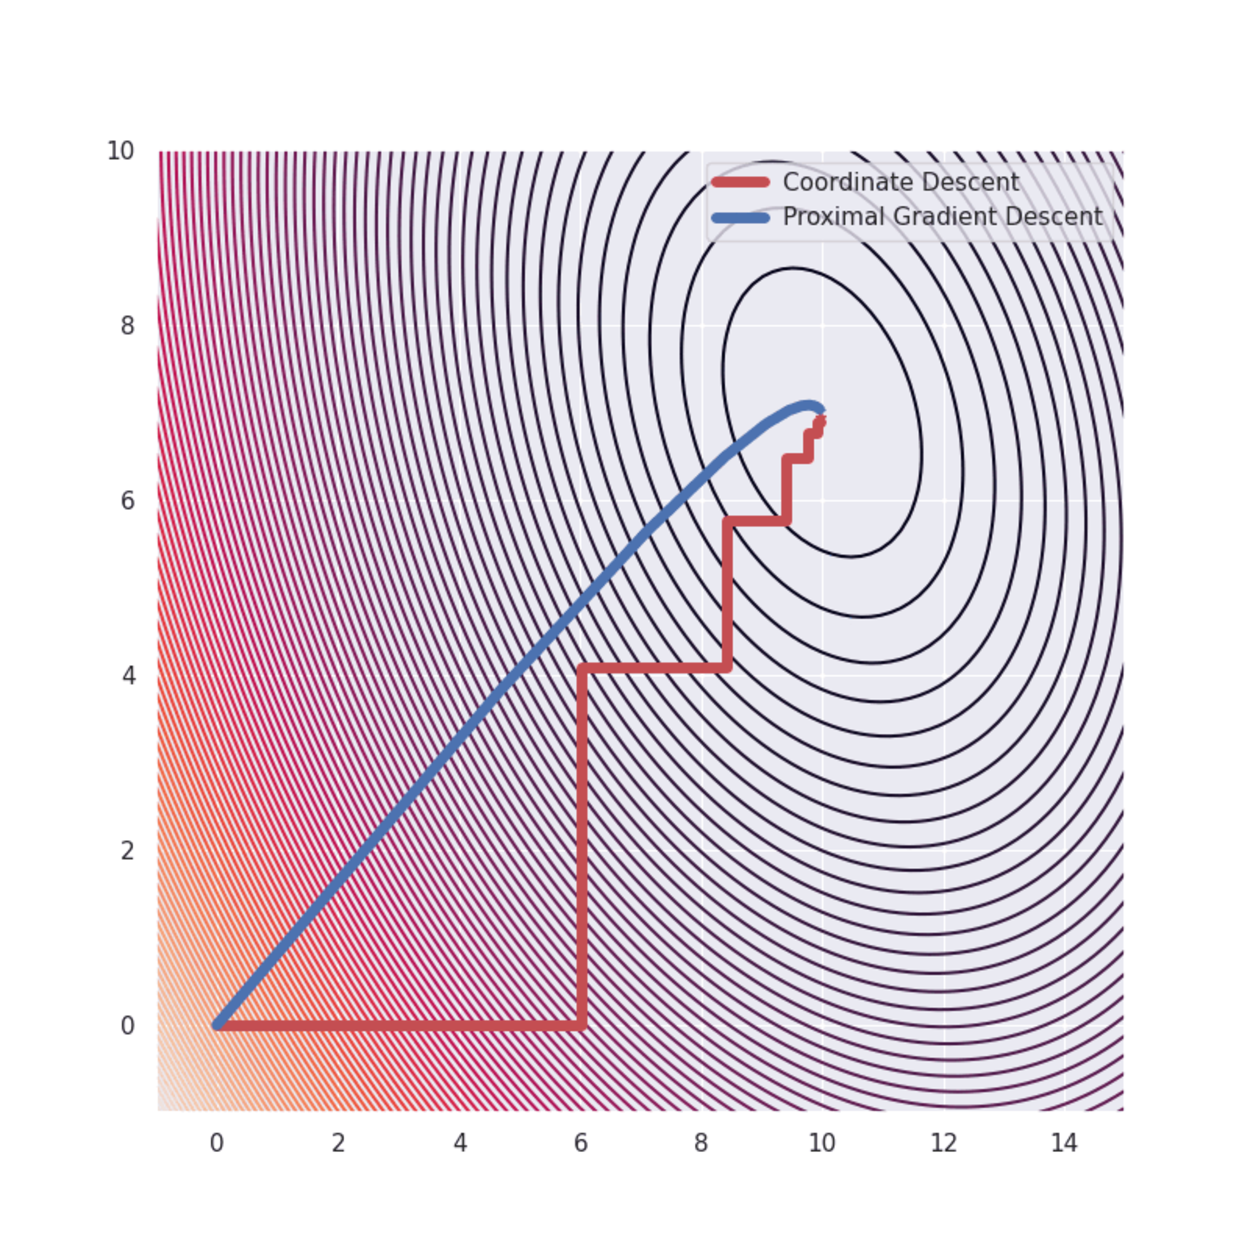
\includegraphics[height=3cm,keepaspectratio]{temp12}};
% \tikz[remember picture,overlay]
% \node at ([xshift=-3.5cm,yshift=-8.0cm]current page.north east)
% {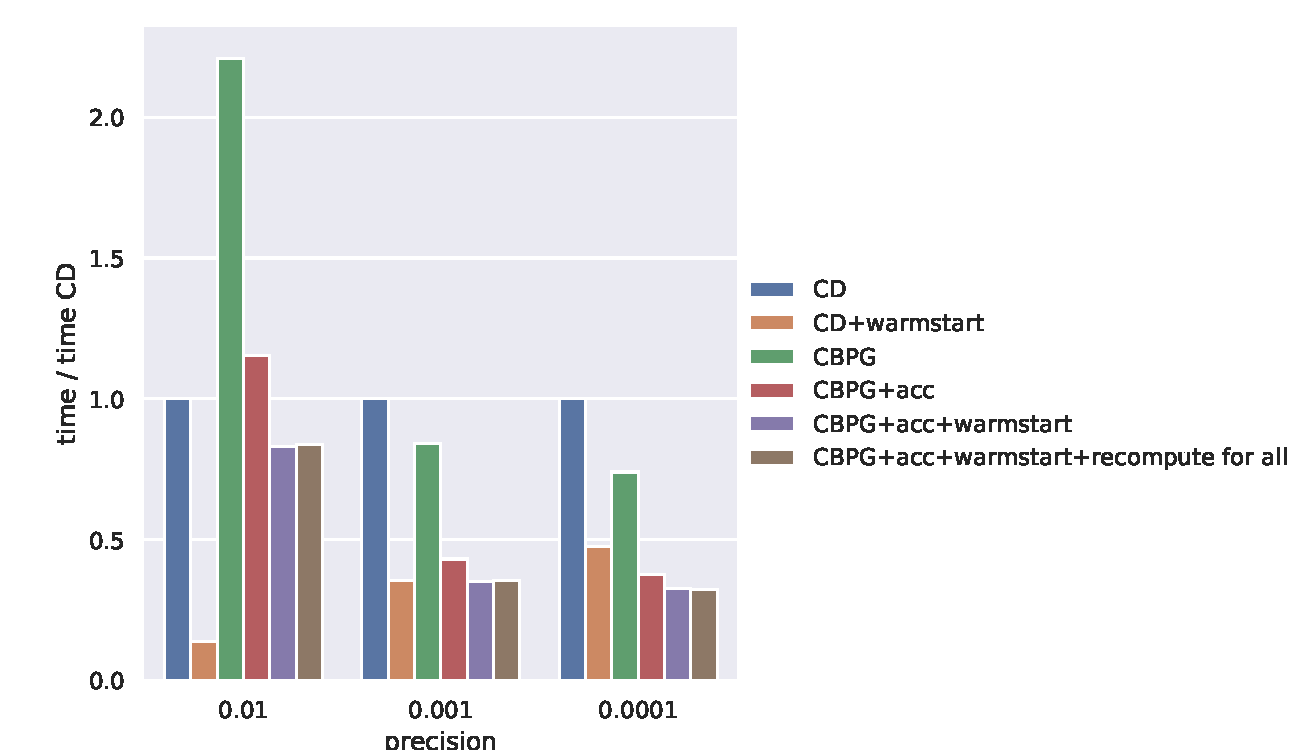
\includegraphics[height=3cm,keepaspectratio,
% clip, trim={0cm 0cm 10cm 0cm}]{barplot_genom_factor20.pdf}};
% \tikz[remember picture,overlay]
% \node at ([xshift=-6cm,yshift=-6cm]current page.north east)
% {
%     \begin{tikzpicture}[scale=.3]
%         \begin{axis}[
%                 xlabel=$x$,
%                 ylabel=$y$,
%                 xmin=-1.5,   xmax=1.5,
%                 ymin=-1,   ymax=1.5,
%             ]
%         \addplot[mark = none, samples at={-1.5,0,1.5}, color=red]{abs(x)};
%         \foreach \fact in {-.8, -.6, -.2, 0, .2, .6, .8} {
%             \addplot[dashed, mark = none, color=blue]{\fact*x};
%             }
%         \end{axis}
%         \end{tikzpicture}
% };
% \tikz[remember picture,overlay]
% \node at ([xshift=-2cm,yshift=-5cm]current page.north east)
% {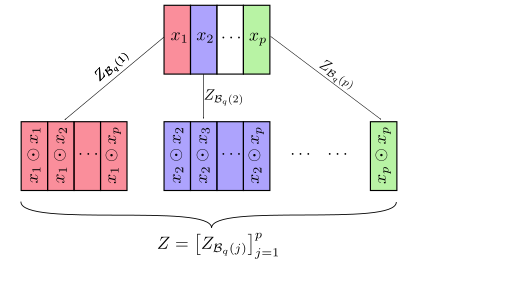
\includegraphics[height=2cm,keepaspectratio]{building_interactions.pdf}};

% \end{frame}

%%%%%%%%%%%%%%%%%%%%%%%%%%%%%%%%%%%%%%%%%%%%%%%%%%%%%%%%%%%%%%%%%%%%%%%%%%%%%%%
%%%%%%%%%%%%%%%%%%%%%%%%%%%%%%%%%%%%%%%%%%%%%%%%%%%%%%%%%%%%%%%%%%%%%%%%%%%%%%%
\section*{Introduction}
\label{sec:Introduction}
%%%%%%%%%%%%%%%%%%%%%%%%%%%%%%%%%%%%%%%%%%%%%%%%%%%%%%%%%%%%%%%%%%%%%%%%%%%%%%%
%%%%%%%%%%%%%%%%%%%%%%%%%%%%%%%%%%%%%%%%%%%%%%%%%%%%%%%%%%%%%%%%%%%%%%%%%%%%%%%
\subsection*{Linear model with penalties}
\begin{frame}{Introduction}{The Linear Model}
We denote $X = [x_1,\dots, x_p] \in \bbR^{n \times p}, y \in \bbR^n$ and
$\beta \in \bbR^p$ such that $y\simeq X\beta$ \\

\textbf{Ordinary least squares}:
\begin{align*}
    \hat\beta^{ls}
    =
    \argmin_{\beta\in\bbR^p}
    \frac{1}{2n}\|y-X\beta\|_2^2
    \Longleftrightarrow
    \textcolor{red}{
    \hat \beta^{ls} = (X^\top X)^{-1}X^\top y }
\end{align*}
Challenge with high dimension:
\begin{itemize}
\item if $p>n$ we lose the uniqueness,
\begin{onlyenv}<2>
    \begin{itemize}
        \item  \color{red}{make the problem strictly convex.}
    \end{itemize}
\end{onlyenv}
\item $X^\top X$ may be ill conditioned
($\kappa = \frac{\text{largest singular value}}{
    \text{smallest singular value}} \gg 1 $ )
    due to multicolinearity amongst features
\begin{onlyenv}<2->
    \begin{itemize}
        \item \color{red}{Shift spectrum by a small quantity using
        $\ell_2$ penalty}
    \end{itemize}
\end{onlyenv}
\item too many active features is not interpretable (genomics dataset)
\begin{onlyenv}<2->
    \begin{itemize}
        \item \color{red}{Feature selection using $\ell_1$ penalty}
    \end{itemize}
\end{onlyenv}\end{itemize}
\end{frame}

\subsection*{Elastic-Net with interactions}
\begin{frame}{Introduction}{Elastic-Net estimator}
Elastic-Net \footfullcite{Zou_Hastie05} $=$ combination of LASSO \footfullcite{Tibshirani96} and
Ridge\footfullcite{Tikhonov43}:
\begin{block}{Elastic-Net}
Considering tuning parameters $\lambda_1,\lambda_2>0$:
\begin{align*}
    \hat\beta^{enet} \in \argmin_{\beta \in \bbR^p}\frac{1}{2n}\norm{y - X\beta}_2^2
    + \lambda_1 \norm{\beta}_1
    + \frac{\lambda_2}{2} \norm{\beta}_2^2 \enspace
\end{align*}
\end{block}
\begin{onlyenv}<2>
    And if we add the first order interactions to the model:
    \begin{block}{Elastic-Net with interactions}
    The interactions matrix is $Z\in\bbR^{n\times q}$,
     and coefficients are $\Theta\in\bbR^q$.
        \begin{align*}
        \hat\beta^{\textcolor{red}{inter}}
        \in \argmin_{\substack{\beta \in \bbR^p \\ \Theta \in \bbR^q}}
        \tfrac{1}{2n}\norm{y - X\beta - \textcolor{red}{Z\Theta}}_2^2
        & + \lambda_{\beta,\ell_1} \norm{\beta}_1
        + \tfrac{\lambda_{\beta, \ell_2}}{2} \norm{\beta}_2^2 \\
        & \textcolor{red}{ ~ + \lambda_{\Theta,\ell_1} \norm{\Theta}_1
        + \tfrac{\lambda_{\Theta, \ell_2}}{2} \norm{\Theta}_2^2}
    \end{align*}
\end{block}
\end{onlyenv}
\end{frame}

\begin{frame}{Optimization problem}
\textbf{Our goal:} Solve the Elastic-Net problem
\begin{itemize}
    \item for high dimensional genomics data,
    \item using graphics card parallelization,
    \item at least as fast as currently used algorithms like Coordinate Descent
    with interactions \footfullcite{Bascou_Lebre_Salmon20}.
\end{itemize}
\vspace*{0.5cm}
\begin{onlyenv}<2>
\textbf{Problems:}
    \begin{itemize}
        \item the interactions matrix is not storable in high dimensions,
        \item graphics cards need a lot of data to parallelize operations
        efficiently,
        \item we use solvers, but when do we stop them ?
    \end{itemize}
\end{onlyenv}
\end{frame}

%%%%%%%%%%%%%%%%%%%%%%%%%%%%%%%%%%%%%%%%%%%%%%%%%%%%%%%%%%%%%%%%%%%%%%%%%%%%%%%
%%%%%%%%%%%%%%%%%%%%%%%%%%%%%%%%%%%%%%%%%%%%%%%%%%%%%%%%%%%%%%%%%%%%%%%%%%%%%%%
\section{Gradient Descent solvers}
\label{sec:Gradient_Descent_solvers}
%%%%%%%%%%%%%%%%%%%%%%%%%%%%%%%%%%%%%%%%%%%%%%%%%%%%%%%%%%%%%%%%%%%%%%%%%%%%%%%
%%%%%%%%%%%%%%%%%%%%%%%%%%%%%%%%%%%%%%%%%%%%%%%%%%%%%%%%%%%%%%%%%%%%%%%%%%%%%%%

\begin{frame}{From gradient to coordinate descent
    }{On least squares problem}
Minimize $F(\beta)=\frac{1}{2n}\norm{y - X\beta}_2^2$:
with step $\eta>0$ at epoch $k\in\bbN$,
\begin{block}{Gradient Descent: 1 problem of dimension p}
\[\beta^{k+1} \longleftarrow \beta^k - \eta \LaTeXunderbrace{\frac{1}{n}X^\top (X\beta^k - y)}_{
    \frac{\partial F}{\partial \beta}(\beta^k)
}\]
\end{block}
\begin{onlyenv}<2>
\begin{block}{Coordinate Descent: p problems of dimension 1}
For $j=1,\dots,p$,
\[\beta^{k+1}_j \longleftarrow \beta^k_j - \eta \LaTeXunderbrace{\frac{1}{n}x_j^\top (X\beta^k - y)}_{
    \frac{\partial F}{\partial \beta_j}(\beta^k)
}\]
\end{block}
\end{onlyenv}
\end{frame}

\begin{frame}{Visualization of the behavior: OLS}{Fixed-step size}
\foreach \index in {1, ..., 12}{
    \begin{onlyenv}<\index>
        \begin{figure}
        \centering
        \includegraphics[width=.8\textwidth, clip,
        trim={0cm 0cm 0cm 1.5cm}]{temp\index.pdf}\par%
        \end{figure}
    \end{onlyenv}
}
\end{frame}

\subsection{Proximal operator}
\begin{frame}{And with a non differentiable function?}{Proximal operators}
\[\argmin_{\beta\in \bbR^p}
\LaTeXunderbrace{\frac{1}{2n}\norm{y-X\beta}_2^2}_{\text{smooth } F(\beta)} +
\LaTeXunderbrace{
    \lambda_1 \norm{\beta}_1 + \frac{\lambda_2}{2}\norm{\beta}_2^2}_{
\text{non-smooth separable } g(\beta)
}\]
\begin{onlyenv}<2>
Gradient descent on $F$ with step $\eta>0$:
\[\beta^{k+1} \longleftarrow \beta^k - \eta \frac{1}{n}X^\top(X\beta - y)\]
\end{onlyenv}

\begin{onlyenv}<3>
\textcolor{red}{Proximal} Gradient descent on $F+g$ with step $\eta>0$:
\[\beta^{k+1} \longleftarrow
\textcolor{red}{\prox_{\eta g}\big( }\beta^k -
 \textcolor{red}{\eta} \frac{1}{n}X^\top(X\beta^k - y)\textcolor{red}{\big)}\]

\begin{block}{Proximal operator}
Let $f$ a convex proper closed function, for $\mu>0$:
\begin{align*}
\prox_{\mu f}(u) = \argmin_{x\in\dom f}\left\{
    f(x) + \frac{1}{2\mu}\norm{x-u}_2^2
\right\} \enspace.
\end{align*}
\end{block}
\end{onlyenv}

\end{frame}

\begin{frame}{Proximal operator}{For the Elastic-Net}
\begin{mybox}{Elastic-Net penalty proximal operator}

Let $h(x)=\|x\|_1 + \frac{\gamma}{2}\|x\|_2^2,\ \gamma>0$, we know \footnotemark
 that for $\mu>0$:
\[
\prox_{\mu h}(x) = \dfrac{1}{1 + \mu\gamma}\prox_{\mu \|\cdot\|_1}(x) =
\dfrac{\sign(x)}{1 + \mu\gamma}(|x| - \mu)_+
\]
where $\sign(x)(\abs{x} - \mu)_+$ is the soft thresholding operator
$\ST(x,\mu)$.

\end{mybox}

\begin{figure}[h]
\centering
% \usetikzlibrary{arrows}
% \begin{tikzpicture}[>=stealth', scale=.7,]
% 	\tkzInit[xmin=-5,xmax=5,
% 			 ymin=-5,ymax=5,
% 			 xstep=2,ystep=2]
% 	\tkzLabelY[orig=false]
% 	\tkzLabelX[orig=false]
% 	\tkzDrawX
% 	\tkzDrawY
% 	\tkzFct[domain=-5:5,color=blue,very thick]{\x}
% 	\node[above] at (2,2.5) {$y=x$};
% 	\tkzFct[domain=2:5,color=red,very thick]{\x-2}
% 	\tkzFct[domain=-5:-2,color=red,very thick]{\x + 2}
% 	\tkzFct[domain=-2:2,color=red,very thick]{0}
% 	\node[above] at (-2,.5) {$y=\mathrm{ST}(x, 2)$};
% \end{tikzpicture}
\includegraphics[width=.4\textwidth]{soft_thresholding}
\end{figure}
\footnotetext{\fullcite[p.~189]{Parikh14}}
\end{frame}

% \begin{frame}{Algorithm with interactions}
% With step sizes the inverse of Lipschitz constants of
% $\frac{1}{2n}\norm{y-X\beta - Z\Theta}_2^2$: $L_X=\frac{\norm{X^\top X}_2}{n}$
% and $L_Z = \frac{\norm{Z^\top Z}_2}{n}$,

% \begin{block}{Alternating minimization}
% \begin{onlyenv}<1>
% \begin{align*}
% \beta^{k+1} &\longleftarrow \frac{1}{1 +
% \frac{1}{L_X} \lambda_{\beta, \ell_2}}
% \mathrm{ST}
% \left(\beta^k - \frac{1}{L_X n}
%  X^\top (X\beta^{k} + Z\Theta^k - y),
% \frac{1}{L_X}\lambda_{\beta, \ell_1}
% \right) \enspace,
% \end{align*}
% \end{onlyenv}
% \begin{onlyenv}<2>
% \begin{align*}
% \beta^{k+1} &\longleftarrow \frac{1}{1 +
% \frac{1}{L_X} \lambda_{\beta, \ell_2}}
% \mathrm{ST}
% \left(\beta^k - \frac{1}{L_X n}
%  X^\top (X\beta^{k} + Z\Theta^k - y),
% \frac{1}{L_X}\lambda_{\beta, \ell_1}
% \right) \enspace, \\
% \textcolor{red}{\Theta}^{k+1} & \longleftarrow \frac{1}{1 +
% \frac{1}{\textcolor{red}{L_Z}} \lambda_{\textcolor{red}{\Theta}, \ell_2}}
% \mathrm{ST}
% \left( \textcolor{red}{\Theta}^k - \frac{1}{\textcolor{red}{L_Z} n}
% \textcolor{red}{Z}^\top (X\beta^{\textcolor{red}{k+1}} + Z\Theta^k - y),
% \frac{1}{\textcolor{red}{L_Z}}\lambda_{\textcolor{red}{\Theta}, \ell_1}
% \right) \enspace.
% \end{align*}
% \end{onlyenv}
% \end{block}
% \end{frame}


\subsection{Accelerations}
\begin{frame}{Accelerate the algorithms}
Possibilities to use accelerations:
\begin{itemize}
    \setlength\itemsep{1em}
    \item Theoretical:
    \begin{itemize}
        \item inertial: heavy ball-like \footfullcite{nesterov27method},
        \item structure of the iterates: Anderson \footfullcite{bertrand2021anderson},
        \item stochastic directions: \footfullcite{nesterov2012efficiency},
        \item structure of the problem: use block updates \footfullcite{Beck17}.
    \end{itemize}
    \item Computational:
    \begin{itemize}
        \item \texttt{Numba} library: \footfullcite{lam2015numba},
        \item GPU acceleration with \texttt{CUDA}.
    \end{itemize}
\end{itemize}
\end{frame}

% \begin{frame}[fragile]{Why use a GPU ?}{Accelerated PGD on CPU is not very competitive}
%     \begin{columns}
%         \begin{column}{0.55\textwidth}
%             \centering
%             \includegraphics[width=1.5\textwidth]{benchopt_plt}
%            \hfill Benchmark LASSSO problem on CPU (Figure made with
%            the \texttt{BenchOpt} library)
%         \end{column}
%     \end{columns}
% \end{frame}

%%%%%%%%%%%%%%%%%%%%%%%%%%%%%%%%%%%%%%%%%%%%%%%%%%%%%%%%%%%%%%%%%%%%%%%%%%%%%%%
% \begin{frame}[noframenumbering]{The BenchOpt library (digress)}{Results page:
%     a cooperative website}

% \begin{center}
%     \url{https://benchopt.github.io/results}
% \end{center}
% \begin{figure}[h]
%     \centering
%     \includegraphics[width=.9\textwidth]{benchopt_res_index}
% \end{figure}
% \end{frame}
%%%%%%%%%%%%%%%%%%%%%%%%%%%%%%%%%%%%%%%%%%%%%%%%%%%%%%%%%%%%%%%%%%%%%%%%%%%%%%%

\begin{frame}[fragile]{Why use a GPU ?}{Accelerated PGD on CPU is not very competitive}
    \begin{columns}
        \begin{column}{0.55\textwidth}
            \centering
            \includegraphics[width=1\textwidth]{benchopt_plt}
           \hfill Benchmark LASSSO problem on CPU (Figure made with
            \texttt{BenchOpt} library \footnotemark)
        \end{column}
        \begin{column}{0.55\textwidth}
            \centering
            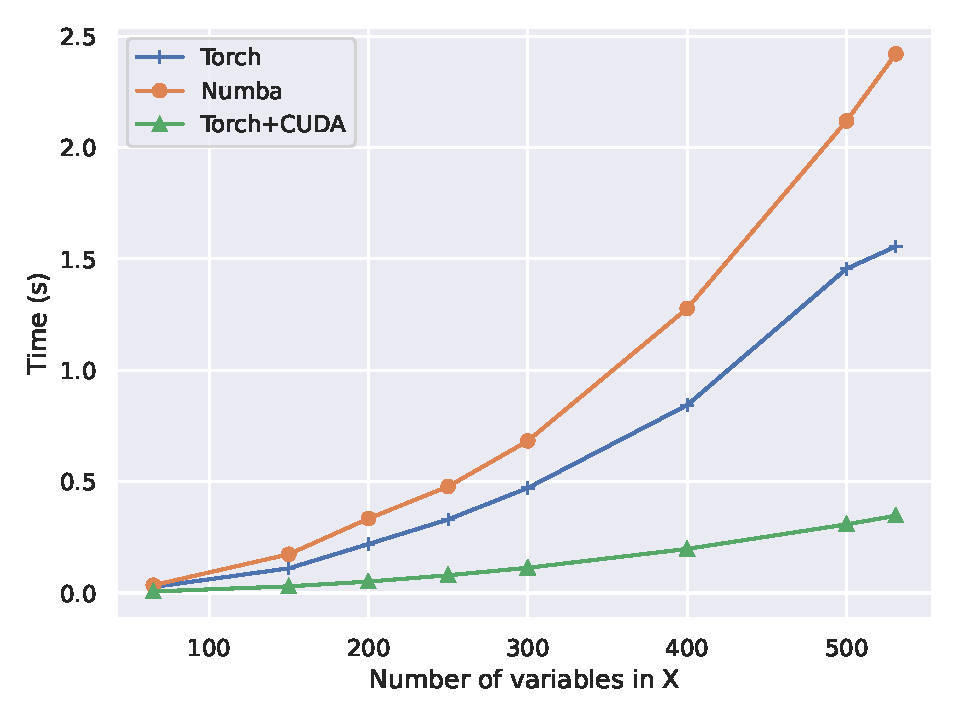
\includegraphics[width=1\textwidth]{benchmark_prod_Zbeta}
            \hfill Benchmark product $Z\Theta$
        \end{column}
    \end{columns}
    \medskip
\begin{onlyenv}<2>
    And it is \textbf{easy} with \texttt{PyTorch}:
    \begin{minted}[
        frame=lines,
        framesep=2mm,
        baselinestretch=1.2,
        bgcolor=LightGray]
        {python}
        A = torch.tensor([1., 2.], device="cuda")
        B = torch.tensor([1., 2.]).to("cuda")
    \end{minted}
\end{onlyenv}
\footnotetext{\url{https://benchopt.github.io}}
\end{frame}


\subsection{First order interactions and blocks}
\begin{frame}{Building the interactions}{First order interactions by block}
See the interactions as blocks generated from $X=[x_1|\dots|x_p]$:
\begin{figure}[h]
    \centering
    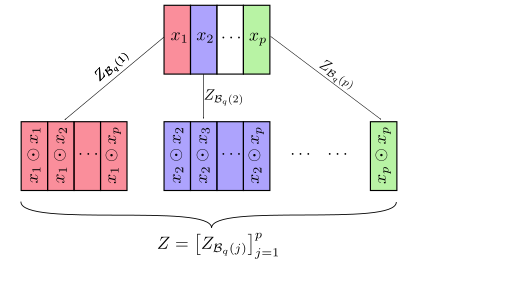
\includegraphics[width=.9\textwidth]{building_interactions.pdf}
\end{figure}
\end{frame}

\begin{frame}{Cyclic Block Proximal Gradient Descent}
$\Longrightarrow$ exploit the blocks in $Z$ for the updates on $\Theta$
\footfullcite{massias2019sparse,Beck17}.

\begin{block}{CBPG update on $\Theta$}
For $j=1,\dots,p$:
\begin{align*}
\textcolor{red}{\Theta}_{\textcolor{red}{\branch{q}{j}}}^{k+1} & \longleftarrow \frac{1}{1 +
\frac{1}{\textcolor{red}{L_j}} \lambda_{\textcolor{red}{\Theta}, \ell_2}}
\mathrm{ST}
\left( \textcolor{red}{\Theta}_{\textcolor{red}{\branch{q}{j}}}^k - \frac{1}{\textcolor{red}{L_j} n}
\textcolor{red}{Z}_{\textcolor{red}{\branch{q}{j}}}^\top (X\beta^{\textcolor{red}{k+1}} + Z\Theta^k - y),
\frac{1}{\textcolor{red}{L_j}}\lambda_{\textcolor{red}{\Theta}, \ell_1}
\right)
\end{align*}
\end{block}

\begin{itemize}
    \item steps $L_j=\tfrac{\|Z_{\branch{q}{j}}^\top Z\|_2}{n}$, $j=1,\dots,p$ Lipschitz constants for each block
    \item computed with iterative method (L\'{a}nczos algorithm \footfullcite{lanczos1952solution}).
\end{itemize}
\end{frame}


%%%%%%%%%%%%%%%%%%%%%%%%%%%%%%%%%%%%%%%%%%%%%%%%%%%%%%%%%%%%%%%%%%%%%%%%%%%%%%%
%%%%%%%%%%%%%%%%%%%%%%%%%%%%%%%%%%%%%%%%%%%%%%%%%%%%%%%%%%%%%%%%%%%%%%%%%%%%%%%
\section{Stopping criterion}
\label{sec:Stopping_criterion}
%%%%%%%%%%%%%%%%%%%%%%%%%%%%%%%%%%%%%%%%%%%%%%%%%%%%%%%%%%%%%%%%%%%%%%%%%%%%%%%
%%%%%%%%%%%%%%%%%%%%%%%%%%%%%%%%%%%%%%%%%%%%%%%%%%%%%%%%%%%%%%%%%%%%%%%%%%%%%%%
% \begin{frame}{Running our solvers: until when?}{KKT conditions}
% For an objective $f$ penalized with $m>0$ inequality constraints
% $h_i,\ i=1,\dots,m$ the minimization problem writes:
% \begin{align*}
%     \min_{x\in\dom f} f(x)\ s.t.\ h_i(x)\leq 0,\ i=1,\dots,m\enspace.
% \end{align*}
% This can be rewritten as minimizing the following Lagrangian function with
% $\mu_1,\dots,\mu_m\in \bbR$:
% \begin{align*}
%     \cL(x, \mu_1,\dots,\mu_m) = f(x) + \sum_{i=1}^m \mu_i h_i(x)
%     \enspace.
% \end{align*}

% \mytheorem{KKT conditions}{

% At the optimum $x^*$
%     \begin{enumerate}
%         \item $0\in \partial f(x^*) + \sum_{i=1}^m \mu_i \partial h_i(x^*)$
%         (stationarity),
%         \item $\forall i\in [m],\ \mu_i h_i(x^*)=0$ (complementary slackness),
%         \item $\forall i\in [m],\ \mu_i>0$ and $h_i(x^*) \leq 0$ (feasibility).
%     \end{enumerate}
% }
% \end{frame}

\subsection{Subgradients}
\begin{frame}{With non-differentiable functions}{Subgradients}
Let $f:\,\bbR^n\rightarrow \bbR$ be a real convex function.
\begin{block}{Subdifferential $\partial f$}
    At $x_0\in\bbR^n$:
    \begin{align*}
        \partial f(x_0) = \left\{ u \in \bbR^n,\ f(x) \geq f(x_0) +
        \langle u, x-x_0\rangle\ \forall x\in \bbR^n\right\}
    \end{align*}
\end{block}
\begin{columns}
\begin{column}{.4\textwidth}
\textbf{Example: } The absolute value at the origin
\[\partial \abs{\cdot}_{|x} =
\begin{cases}
    \{-1\}, & \text{ if } x <0\\
    \{1\}, & \text{ if }x>0 \\
    [-1, 1],& \text{ if } x=0 \end{cases}
\]
\end{column}
\begin{column}{.6\textwidth}
\begin{figure}[h]
    \centering
\begin{tikzpicture}[scale=.6]
\begin{axis}[
        xlabel=$x$,
        ylabel=$y$,
        xmin=-1.5,   xmax=1.5,
        ymin=-1,   ymax=1.5,
    ]
\addplot[mark = none, samples at={-1.5,0,1.5}, color=red]{abs(x)};
\addlegendentry{$\abs{x}$};
\foreach \fact in {-.8, -.6, -.2, 0, .2, .6, .8} {
    \addplot[dashed, mark = none, color=blue]{\fact*x};
    }
\addlegendentry{subtangents at $(0,0)$};
\end{axis}
\end{tikzpicture}
\end{figure}
\end{column}
\end{columns}
\end{frame}

\subsection{KKT violation}
\begin{frame}{KKT violation criterion}
Elastic-Net: $\argmin_{\beta\in\bbR^p}
        \frac{1}{2n} \|y - X\beta\|^2_2 + \lambda_1 \|\beta\|_1 +
        \frac{\lambda_2}{2}\|\beta\|^2_2 = \argmin F_{enet}(\beta).$

\begin{block}{KKT violation}
Our criterion: how much do we violate the KKT conditions:
\begin{align*}
    d_{\norm{\cdot}_\infty}(0, \partial F_{enet}(\beta)) \leq \epsilon
    \Longleftrightarrow \inf_{g\in\partial F_{enet}(\beta)}\norm{g}_\infty
    \leq \epsilon
\end{align*}
Splitting along the coordinates, denoting $r=y-X\beta$:
\begin{align*}
d\left(0, \frac{1}{n}X_j^\top(X\beta - y)
+ \lambda_1 \partial_{\abs{\cdot}}(\beta_j)
+ \lambda_2 \beta_j  \right) =
\frac{1}{n} \left| \mathrm{ST}\left( X_j^\top r - n \lambda_2 \beta_j
, n\lambda_1 \right) \right|
\end{align*}
\end{block}
\end{frame}

%%%%%%%%%%%%%%%%%%%%%%%%%%%%%%%%%%%%%%%%%%%%%%%%%%%%%%%%%%%%%%%%%%%%%%%%%%%%%%%
%%%%%%%%%%%%%%%%%%%%%%%%%%%%%%%%%%%%%%%%%%%%%%%%%%%%%%%%%%%%%%%%%%%%%%%%%%%%%%%
\section{Application to datasets}
\label{sec:application_to_datasets}
%%%%%%%%%%%%%%%%%%%%%%%%%%%%%%%%%%%%%%%%%%%%%%%%%%%%%%%%%%%%%%%%%%%%%%%%%%%%%%%
%%%%%%%%%%%%%%%%%%%%%%%%%%%%%%%%%%%%%%%%%%%%%%%%%%%%%%%%%%%%%%%%%%%%%%%%%%%%%%%

%%%%%%%%%%%%%%%%%%%%%%%%%%%%%%%%%%%%%%%%%%%%%%%%%%%%%%%%%%%%%%%%%%%%%%%%%%%%%%%
\subsection{Simulated datasets}
\label{subsec:simulated_datasets}
%%%%%%%%%%%%%%%%%%%%%%%%%%%%%%%%%%%%%%%%%%%%%%%%%%%%%%%%%%%%%%%%%%%%%%%%%%%%%%%

% \begin{frame}{Simulated datasets}{Building the simulation}

% \begin{onlyenv}<1->
% \begin{block}{Signal to noise ratio}
% For a random centered gaussian noise $\varepsilon$ of variance $\sigma^2$
% \[\mathrm{SNR} = \frac{\var(y)}{\sigma^2}\enspace.\]
% \end{block}
% \end{onlyenv}

% \begin{onlyenv}<1>
%     \textbf{LASSO:} $ \frac{1}{2n}\norm{y-X\beta - Z\Theta}_2^2
%     + \lambda_{1}\norm{\beta}_1 + \lambda_{2}\norm{\Theta}_1$
% \begin{block}{Max $\ell_1$ penalty}
% The maximum $\ell_1$ penalty is defined such that:
% \begin{align*}
%     \forall \lambda > \lambda_{\max},\  \hat\beta=0_p \text{ and } \hat\Theta=0_q
% \end{align*}
% It is computed using \footfullcite{Fercoq_Gramfort_Salmon15}:
% \begin{align*}
% 	\lambda_{\max} = \max\left(\frac{\norm{X^\top y}_\infty}{n},
% 							\frac{\norm{Z^\top y}_\infty}{n}\right)
% \end{align*}
% \end{block}
% \end{onlyenv}

% \end{frame}


%%%%%%%%%%%%%%%%%%%%%%%%%%%%%%%%%%%%%%%%%%%%%%%%%%%%%%%%%%%%%%%%%%%%%%%%%%%%%%%
\begin{frame}{Applications}{Simulated datasets}
$X$ from Gaussian distribution, $n=20000$, $p=500$ (train/test $=75\%/25\%$), $SNR=10$,
$1\%$ of non-zero values in $\beta^*$ and $\Theta^*$.
\begin{itemize}
    \item $\ell_1$ penalty is $\frac{\lambda_{\max}}{\ell_1\ factor}$,
    \item $\ell_2$ penalty is $\frac{\lambda_{\max}}{10}$,
    \item $\epsilon=10^{-3}$ (PGD did not converge for $\ell_1$ factor
    $> 250$).
\end{itemize}
\begin{columns}
\begin{column}{.59\textwidth}
\begin{figure}[h]
    \centering
    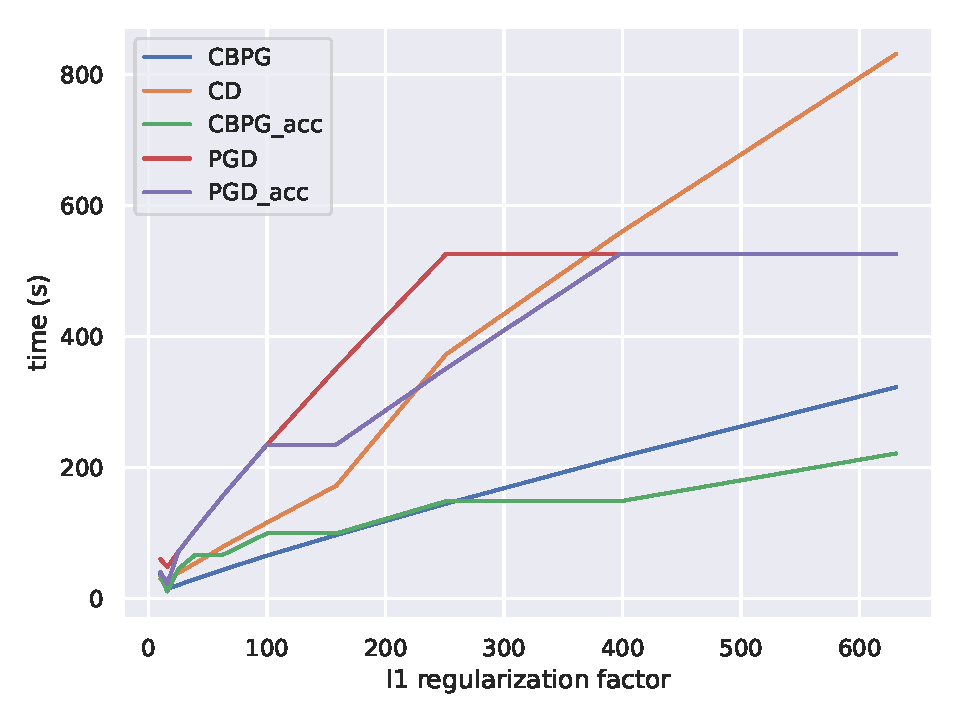
\includegraphics[width=.9\textwidth]{simulated_n20000p500_snr=10_TIME}
\end{figure}
\end{column}
\begin{column}{.4\textwidth}
\begin{itemize}
    \item CD faster at the beginning,
    \item CBPG faster after,
    \item convergence issues with PGD.
\end{itemize}
\end{column}
\end{columns}
\end{frame}
%%%%%%%%%%%%%%%%%%%%%%%%%%%%%%%%%%%%%%%%%%%%%%%%%%%%%%%%%%%%%%%%%%%%%%%%%%%%%%%

%%%%%%%%%%%%%%%%%%%%%%%%%%%%%%%%%%%%%%%%%%%%%%%%%%%%%%%%%%%%%%%%%%%%%%%%%%%%%%%
% \begin{frame}{Applications}{Simulated datasets}
% Same setting for the creation of $X$.
% \begin{itemize}
%     \item $\ell_1$ ratio of $0.9$ \ie $\ell_1$ penalty of $\alpha\ell_{1\ ratio}$ and
%     $\ell_2$ penalty of $\alpha(1-\ell_{1\ ratio})$,
%     \item $\lambda_{\max}$ is divided by $\ell_1$ ratio,
%     \item $\alpha\in[\lambda_{\max}/100, \lambda_{\max}/1.1]$,
%     \item warmstart used to reach $\epsilon=10^{-4}$.
% \end{itemize}

% \begin{figure}
%     \centering
%     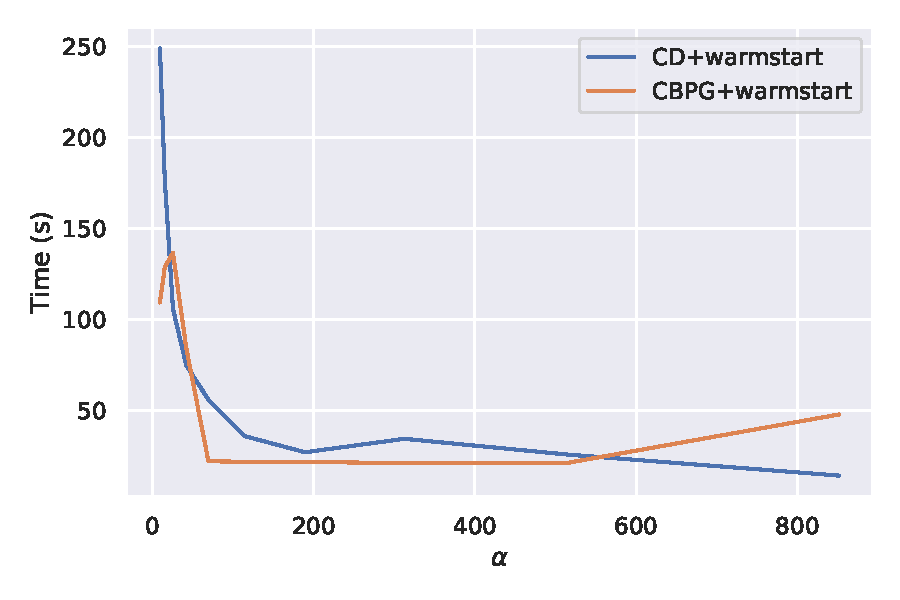
\includegraphics[scale=.6, clip, trim={0cm 0cm 15cm .5cm}]{simu_ratio09}
% \end{figure}

% \end{frame}
%%%%%%%%%%%%%%%%%%%%%%%%%%%%%%%%%%%%%%%%%%%%%%%%%%%%%%%%%%%%%%%%%%%%%%%%%%%%%%%


%%%%%%%%%%%%%%%%%%%%%%%%%%%%%%%%%%%%%%%%%%%%%%%%%%%%%%%%%%%%%%%%%%%%%%%%%%%%%%%
\subsection{Genomics dataset}
\label{subsec:genomics_dataset}
%%%%%%%%%%%%%%%%%%%%%%%%%%%%%%%%%%%%%%%%%%%%%%%%%%%%%%%%%%%%%%%%%%%%%%%%%%%%%%%

%%%%%%%%%%%%%%%%%%%%%%%%%%%%%%%%%%%%%%%%%%%%%%%%%%%%%%%%%%%%%%%%%%%%%%%%%%%%%%%
\begin{frame}{Genomics dataset}{Presentation}
\begin{itemize}
    \item $n=19393$ samples (genes) and $531$ features ($141246$ interactions
    \ie way too much!)\footfullcite{Bessiere_Taha_Petitprez_Vandel_Marin_Brehelin_Lebre_Lecellier}
    \item $y$ is the gene expression in one patient (the first)
\end{itemize}

\begin{columns}
\begin{column}{.5\textwidth}
    \begin{figure}
        \centering
    \begin{onlyenv}<1>
        \includegraphics[width=\textwidth, clip, trim={1.2cm 0 1cm 0}]{Gram_matrix_genom}
        \caption*{Correlation matrix of $X$}
    \end{onlyenv}
    \begin{onlyenv}<2>
        \includegraphics[width=\textwidth, clip, trim={1.2cm 0 1cm 0}]{Gram_matrix_genom_60}
        \caption*{Correlation matrix of the first $60$ features}
    \end{onlyenv}
    \end{figure}
\end{column}
\begin{column}{.6\textwidth}
    \begin{itemize}
        \item $20$ features for (di)nucleotides in Core region
        \item $20$ Distal Upstream region promoter
        \item $20$ in Distal Downstream region promoter
        \item $471$ for motif scores in the Core region (in $[0,1]$
        close to $1$)
    \end{itemize}
\end{column}
\end{columns}
\end{frame}
%%%%%%%%%%%%%%%%%%%%%%%%%%%%%%%%%%%%%%%%%%%%%%%%%%%%%%%%%%%%%%%%%%%%%%%%%%%%%%%
%%%%%%%%%%%%%%%%%%%%%%%%%%%%%%%%%%%%%%%%%%%%%%%%%%%%%%%%%%%%%%%%%%%%%%%%%%%%%%%
\begin{frame}{Genomics dataset}{What we need to know (numerically)}
\begin{columns}
\begin{column}{.5\textwidth}
    \begin{figure}[h]
        \centering
        \includegraphics[width=1.2\textwidth,
        clip, trim={0cm 0cm 0cm 1.5cm}]{condition_number_genom}
        \caption*{Very ill conditioned data (by block)
        }
    \end{figure}
\end{column}
\hfill
\begin{column}{.5\textwidth}
    \begin{figure}[h]
        \centering
        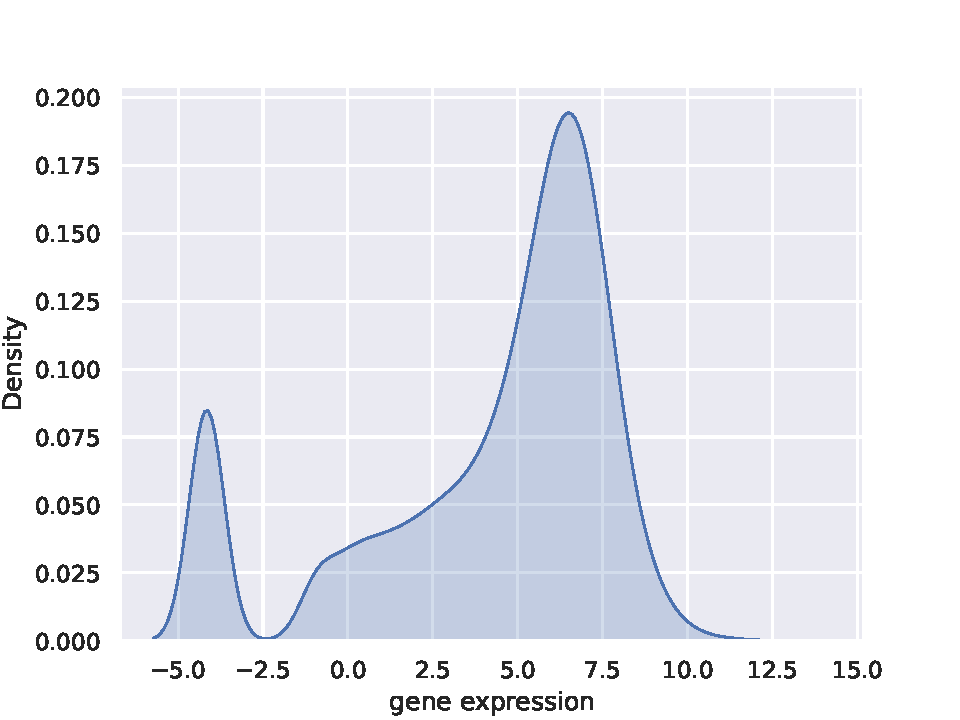
\includegraphics[width=1.1\textwidth,
        clip, trim={0cm 0cm 0cm 1.5cm}]{distrib_gene_expression}
        \caption*{Preprocessing on $y$: $\log$-transformed for unimodaltiy
        (shifted by $\epsilon>0$):
        }
    \end{figure}
\end{column}
\end{columns}
\end{frame}
%%%%%%%%%%%%%%%%%%%%%%%%%%%%%%%%%%%%%%%%%%%%%%%%%%%%%%%%%%%%%%%%%%%%%%%%%%%%%%%
%%%%%%%%%%%%%%%%%%%%%%%%%%%%%%%%%%%%%%%%%%%%%%%%%%%%%%%%%%%%%%%%%%%%%%%%%%%%%%%
\begin{frame}{Genomics dataset}{Solver on path}
Running our solvers \textbf{considering warmstarts}:
\begin{itemize}
    \item $\ell_1$ penalty: $10$ $\log$-spaced values on a grid
    from $\lambda_{\max}$ to $\lambda_{\max}/100$
    \item $\ell_2$ penalty: set to $20\lambda_{\ell_1, \max}$
\end{itemize}
\begin{figure}[h]
    \centering
    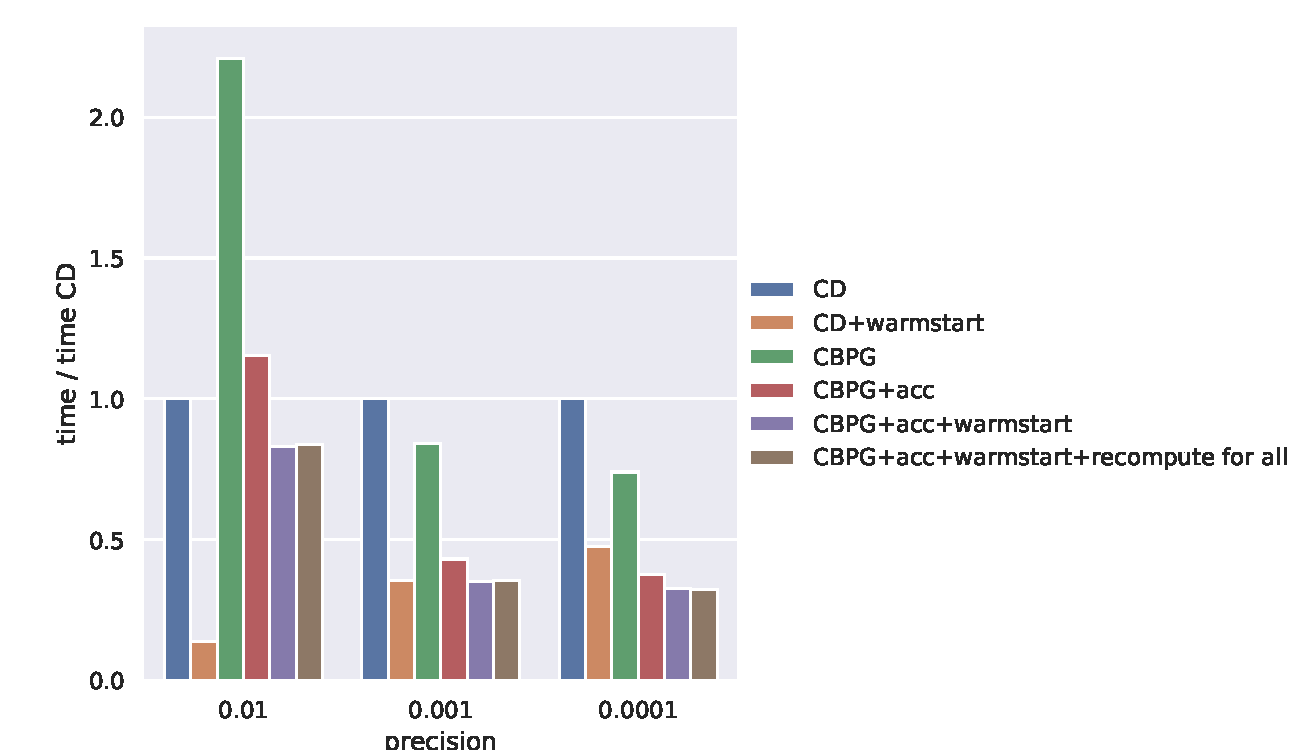
\includegraphics[width=.8\textwidth]{barplot_genom_factor20}
\end{figure}
\begin{itemize}
    \item All resulting in the same active features.
\end{itemize}
\end{frame}
%%%%%%%%%%%%%%%%%%%%%%%%%%%%%%%%%%%%%%%%%%%%%%%%%%%%%%%%%%%%%%%%%%%%%%%%%%%%%%%


\begin{frame}{Conclusion}
\textbf{In short:}
\begin{itemize}
    \item \textbf{It is possible} to be faster using GPU and inertial
    acceleration \dots
    \item<2-> \textbf{but} there is a tradeoff with the precision.
    \item<3-> CBPG algorithms needs more epochs than CD but compute them faster.
\end{itemize}

\medskip
\begin{onlyenv}<4>
\textbf{Possible leads:}
\begin{itemize}
    \item Consider other types of accelerations,
    \item Compute more precise convergence rates for the KKT violation
    criterion.
    \item Keep working on the \texttt{BenchOpt} library.
\end{itemize}
\end{onlyenv}
\end{frame}

%%%%%%%%%%%%%%%%%
% Biblio
%%%%%%%%%%%%%%%%%

%%%%%%%%%%%%%%%%%%%%%%%%%%%%%%%%%%%%%%%%%%%%%%%%%%%%%%%%%%%%%%%%%%%%%%%%%%%%%%%
\begin{frame}[allowframebreaks,noframenumbering]
    \frametitle{References}
    \footnotesize
    \printbibliography
\end{frame}
%%%%%%%%%%%%%%%%%%%%%%%%%%%%%%%%%%%%%%%%%%%%%%%%%%%%%%%%%%%%%%%%%%%%%%%%%%%%%%


\begin{frame}[plain,noframenumbering]
	\standoutpage{\bfseries\huge Thank you for your attention!}
\end{frame}


\appendix
%%%%%%%%%%%%%%%%%%%%%%%%%%%%%%%%%%%%%%%%%%%%%%%%%%%%%%%%%%%%%%%%%%%%%%%%%%%%%%%
\begin{frame}[noframenumbering]{The BenchOpt library}{Results page:
    a cooperative website}

\begin{center}
    \url{https://benchopt.github.io/results}
\end{center}
\begin{figure}[h]
    \centering
    \includegraphics[width=.9\textwidth]{benchopt_res_index}
\end{figure}
\end{frame}
%%%%%%%%%%%%%%%%%%%%%%%%%%%%%%%%%%%%%%%%%%%%%%%%%%%%%%%%%%%%%%%%%%%%%%%%%%%%%%%
%%%%%%%%%%%%%%%%%%%%%%%%%%%%%%%%%%%%%%%%%%%%%%%%%%%%%%%%%%%%%%%%%%%%%%%%%%%%%%%
\begin{frame}[noframenumbering]{The BenchOpt library}{Creating a filter for system informations}
\centering
\includegraphics[width=1.2\textwidth]{benchopt_filter}
\end{frame}
%%%%%%%%%%%%%%%%%%%%%%%%%%%%%%%%%%%%%%%%%%%%%%%%%%%%%%%%%%%%%%%%%%%%%%%%%%%%%%%
%%%%%%%%%%%%%%%%%%%%%%%%%%%%%%%%%%%%%%%%%%%%%%%%%%%%%%%%%%%%%%%%%%%%%%%%%%%%%%%
\begin{frame}[noframenumbering]{The BenchOpt library}{Filter for mobile devices}
\centering
\includegraphics[width=.8\textwidth]{mobile_filter}
\end{frame}
%%%%%%%%%%%%%%%%%%%%%%%%%%%%%%%%%%%%%%%%%%%%%%%%%%%%%%%%%%%%%%%%%%%%%%%%%%%%%%%
%%%%%%%%%%%%%%%%%%%%%%%%%%%%%%%%%%%%%%%%%%%%%%%%%%%%%%%%%%%%%%%%%%%%%%%%%%%%%%%
\begin{frame}[noframenumbering]{The BenchOpt library}{Interactive results}
\begin{onlyenv}<1>
\centering
\includegraphics[width=\textwidth,
clip, trim={0cm 38cm 0cm 0cm}]{benchopt_results}
\end{onlyenv}
\begin{onlyenv}<2>
\begin{figure}
\centering
\includegraphics[width=.7\textwidth,
clip, trim={0cm 0cm 0cm .3cm}]{ols_benchopt}
\end{figure}
\end{onlyenv}
\end{frame}
%%%%%%%%%%%%%%%%%%%%%%%%%%%%%%%%%%%%%%%%%%%%%%%%%%%%%%%%%%%%%%%%%%%%%%%%%%%%%%%
\end{document}
